\documentclass[a4paper]{scrartcl}

% input encoding
\usepackage[utf8]{inputenc}

% new german spelling
\usepackage[ngerman]{babel}

% choose font
\usepackage[T1]{fontenc}
\usepackage{lmodern}
\usepackage{dsfont}

% KOMA-Script options
\KOMAoptions{%
  parskip=full,%
  fontsize=12pt,%
  DIV=calc}

% color and images
\usepackage{xcolor}
\usepackage{graphicx}
\usepackage{wrapfig}
\usepackage{subcaption}
\captionsetup{compatibility=false}

% SI units 
\usepackage{siunitx} 

% quotes
\usepackage[german=guillemets]{csquotes}

% math
\usepackage{amsmath}
\usepackage{amssymb}
\usepackage{amsfonts} 

% set special behaviour for hyperlinks in pdfs
\usepackage[breaklinks=true]{hyperref}

% tables don't appear anywhere
\usepackage{float}


% other useful packages 
\usepackage{enumitem} 
\usepackage{cancel} 

\begin{document}
\title{V602: Röntgenemission und -absorption}
\author{Tim Alexewicz (tim.alexewicz@udo.edu), \and Sadiah Azeem (sadiah.azeem@udo.edu)}
\date{Versuchsdurchführung: 05.04.2022}

\maketitle
\thispagestyle{empty}
\newpage
\thispagestyle{empty}
\tableofcontents
\newpage
\setcounter{page}{1}

\section{Ziel}
Das Ziel des Versuches ist es, die Bragg Bedingung zu überprüfen, das Emissionsspektrum einer Cu-Röntgenröhre sowie das Absorptionsspektrum, bzw. die K-Kante und Abschirmungskonstante von fünf verschiedenen Materialien zu ermitteln.

\section{Theorie}
Röntgenstrahlung entsteht, wenn ein freies Elektron auf eine Anode einschlägt. Die Röntgenstrahlung eines Anodenmaterials ist durch ihre charakteristische Röntgenstrahlung sowie dem kontinuierlichen Bremsspektrum dessen charakterisiert. Bremsstrahlung entsteht durch die Wechselwirkung zwischen dem Elektron und dem Atomkern. Dabei wird ein Photon, auch Röntgenquant genannt, vom Elektron emittiert. Da das Elektron seine ganze Energie abgeben kann, ist das Bremsspektrum kontinuierlich. Wenn das Elektron vollständig gebremst wird, wandelt sich die kinetische Energie $E_{Kin}=eU$ in Strahlungsenergie $E=h\nu$ um. Die maximale Energie des Elektrons ergibt sich dann aus 
\begin{equation}
  \lambda_{min}=\frac{h\cdot c}{E},
  \label{1}
\end{equation}
der minimalen Wellenlänge.\\
Das charakteristische Spektrum ergibt sich daraus, dass das Anodenmaterial ionisiert wird und dann ein Elektron einer äußeren Schale in die innere Schale wandert, also in einen energetisch niedrigeren Zustand wechselt. Dadurch muss wieder ein Röntgenquant emittiert werden, dessen Energie sich aus der Energiedifferenz 
\begin{equation}
  h\nu=E_{m}-E_{n}
  \label{2}
\end{equation}
der beiden Energieniveaus ermitteln lässt. Diese signifikanten Sprünge ergeben das charakteristische Spektrum des Anodenmaterials, die als scharfe Linien dargestellt werden können. Diese Linien werden mit $K_{\alpha}, K_{\beta}, L_{\alpha}, ...$ bezeichnet, wobei $K,L,M,...$ für die jeweilige Schale steht. Dabei stehen griechische Buchstaben für die Herkunft des äußeren Elektrons, dass in die innere Schale wechselt. In einem Mehrelektronenatom schirmen die Hüllenelektronen die Elektronen der unteren Schalen ab. Dadurch wechselwirkt das äußere Elektron schwächer mit dem Kern und die Bindungsenergie, also die Energie, die benötigt wird, um das Elektron von der n-ten Schale des Atoms zu lösen beträgt
\begin{equation}
  E_{n}=-R_{\infty}z_{eff}^2\cdot\frac{1}{n^2},
  \label{3}
\end{equation}
wobei die Abschirmung in der effektiven Kernladung $z_{eff}=z-\sigma$ enthalten ist, mit der Abschirmkonstante $\sigma$ und der Rydbergenergie $R_{\infty}=13.6\ \si{\eV}$.\\
Zusätzlich können noch der Bahndrehimpuls und der Spin der äußeren Elektronen betrachtet werden. Dabei spaltet sich die charakteristische Kennlinie auf. Diese neue Struktur wird Feinstruktur genannt. Diese kann durch die Sommerfeldsche Feinstrukturformel 
\begin{equation}
  E_{n,j}=-R_{\infty}\left(z^2_{eff,1}\cdot \frac{1}{n^2}+\alpha^2 z^4_{eff,2}\cdot\frac{1}{n^3}\left(\frac{1}{j+\frac{1}{2}}-\frac{3}{4n}\right)\right)
  \label{4}
\end{equation}
berechnet werden, mit der Rydbergenergie $R_{\infty}$, der Feinstrukturkonstante $\alpha$, der effektiven Kernladungszahl $z_{eff}$, der Energiequantenzahl $n$ und dem Gesamtdrehimpuls $j$ des Elektrons.
Bei einer Röntgenstrahlung unter $1\ \si{\MeV}$ sind bei der Absorption der Comptoneffekt und der Photoeffekt relevant. Der Absorptionskoeffizient nimmt mit steigender Energie ab und springt, wenn die Photonenergie größer als die Bindungsenergie des Elektrons der nächsten inneren Schale ist. Die Energien der Elektronen 
\begin{equation}
  h\nu_{abs}=E_{n}-E_{\infty},
  \label{5}
\end{equation}
die aus den Schalen $K,L,M,...$ stammen, werden Absorptionskanten genannt. Bei der K-Kante gibt es nur eine Kante, bei L jedoch mehr. In der K-Schale ist $n=1$ und aus der Sommerfeldschen Feinstrukturformel lässt sich die Abschirmkonstante 
\begin{equation}
  \sigma_{K}=Z-\sqrt{\frac{E_{K}}{R_{\infty}}-\frac{\alpha^2 Z^4}{4}}
  \label{6}
\end{equation}
berechnen.\\
Zuletzt lässt sich auch die Wellenlänge der Röntgenstrahlung aus der Bragg-Bedingung
\begin{equation}
  2dsin\theta=n\lambda
  \label{7}
\end{equation}
bestimmen, mit dem Glanzwinkel $\theta$, der gebeugten Wellenlänge $\lambda$ und der Beugungsordnung $n$. Das funktioniert, weil das Röntgenlicht an der Netzebene des Kristalls beugt, aber nur mit dem selben Wellenvektor $\vec k$ austreten kann, wenn es konstruktiv interferieren soll, heißt $\vec p=\hbar\vec k=\hbar\vec k'=\vec p'$, mit $\vec p$ Impuls der einlaufenden Welle und $\vec p'$ Impuls der auslaufenden Welle. 

\section{Versuchsaufbau}
\begin{figure}[H]
\centering
  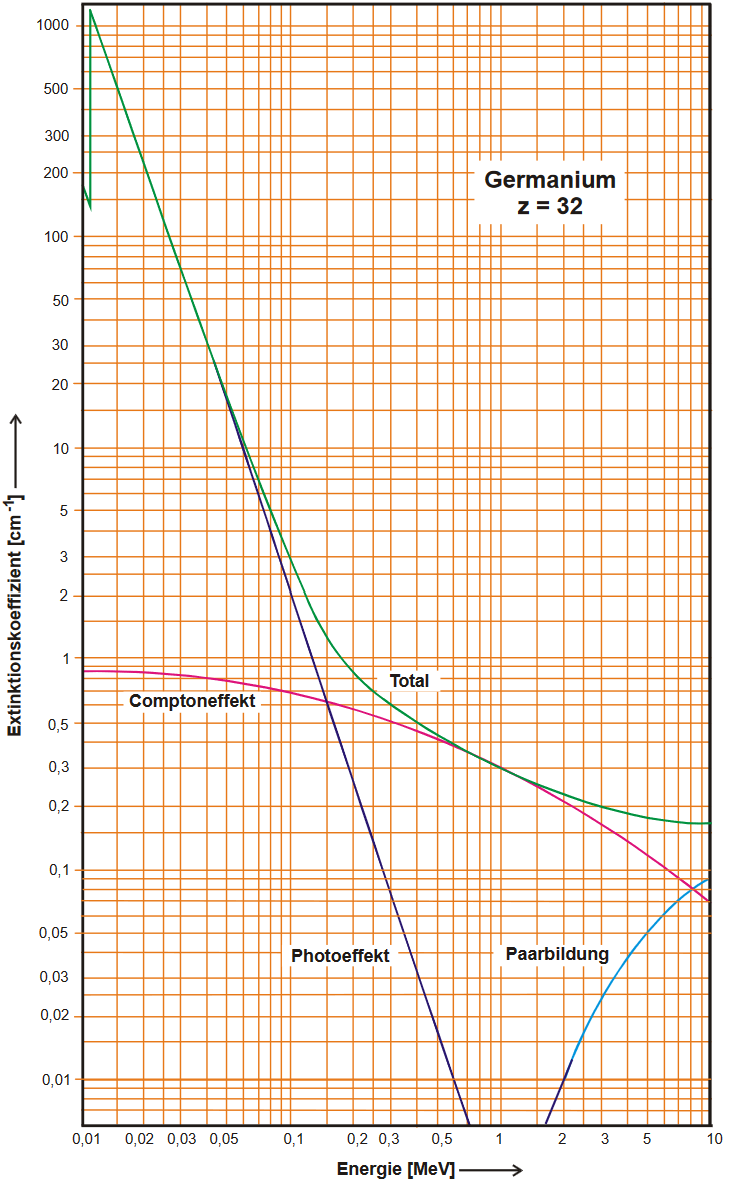
\includegraphics[width=9cm]{1}
  \caption{Das Messgerät}
  \label{fig:1}
\end{figure}
Für das Experiment wird lediglich eine Kuper-Röntgenröhre, ein KBr-kristall und ein Geiger-Müller-Zählrohr benötigt. Das alles ist in dem Gerät aus \autoref{fig:1} geschaltet und kann über einen Rechner gesteuert werden. Die Beschleunigungsspannung wird auf $U=35\ \si{\keV}$ und der Emissionsstrom auf $I=1\ \si{\mA}$ gestellt.

\subsection{Überprüfung der Bragg-Bedingung}
Der KBr-Kristall wird auf einen festen Winkel von $\theta=14^{\circ}$ gestellt. Dann soll das Geiger-Müller-Zählrohr den Winkelbereich zwischen $\alpha_{1}=26^{\circ}$ und $\alpha_{2}=30^{\circ}$ in $\Delta\alpha=0.1^{\circ}$-Schritten mit einer Integrationszeit von $\Delta t=5\ \si{\s}$ pro Winkel die Intensität messen.

\subsection{Emissionsspektrum einer Cu-Röntgenröhre}
Zum Messen des Emissionsspektrums einer Cu-Röntgenröhre wir das Programm auf den 2:1 Koppelmodus gestellt und dann das Röntgenspektrum der Beugungsordnung $n=1$ im Winkelbereich zwischen $4^{\circ}\leq\theta\leq 26^{\circ}$ in $\Delta\alpha=0.2^{\circ}$-Schritten mit Integrationszeit $\Delta t=5\ \si{\s}$ gemessen. 

\subsection{Absorptionsspektrum}
Es sollen fünf Absorber mit Kernladungszahlen $30\leq Z\leq 50$ vor das Geiger-Müller-Zählrohr gesetzt werden und das Absorptionsspektrum in $\Delta\alpha=0.1^{\circ}$-Schritten mit Integrationszeit $\Delta t=20\ \si{\s}$ gemessen werden. Der Winkelbereich ist variabel.

\section{Vorbereitung}
Zur Vorbereitung sollte ermittelt werden, bei welchen Energien in keV die $\mathbf{Cu}-K_{\alpha}$- und $\mathbf{Cu}-K_{\beta}$-Linie zu erwarten ist. Diese liegen bei $E_{\mathbf{Cu}-K_{\alpha}}=8.05 \si{\keV}$ und $E_{\mathbf{Cu}-K_{\beta}}=8.91 \si{\keV}$. Die Glanzwinkel errechnen sich unter der Benutzung von \eqref{1} und \eqref{7} zu $\theta_{\alpha}=13.5^\circ$ und $\theta_{\beta}=12.2^\circ$.
Zusätzlich dazu sollte von Zn, Ge, Br, Rb, Sr und Zr die Absorptionskanten $E_{K}$, der Glanzwinkel $\theta_{K}$ und die Abschirmkonstante $\sigma_{K}$ gefunden werden:
\begin{table}[H]
  \centering
  \begin{tabular}{l|l|l|l|l}
  & Z & $E_{K}$ [keV] & $\theta_{K}$ [$^{\circ}$] & $\sigma_{K}$ \\\hline
  Zn & $30$ & $9.65$ & $11.3$ & $3.56$\\\hline
  Ge & $32$ & $11.10$ & $9.8$ & $3.68$\\\hline
  Br & $35$ & $13.47$ & $8.0$ & $3.85$\\\hline
  Rb & $37$ & $15.80$ & $7.1$ & $3.94$\\\hline
  Sr & $38$ & $16.10$ & $6.7$ & $3.99$\\\hline
  Zr & $40$ & $18.00$ & $6.0$ & $4.09$\\\hline
  \end{tabular}
  \caption{Stoffe, deren Ordnungszahlen, Absorptionskanten, Glanzwinkel und Abschirmkonstanten.}
  \label{tab:1}
\end{table}

\section{Auswertung}
\label{sec:Auswertung}



\subsection{Überprüfung der Bragg-Bedingung}
\label{subsec:bragg}
Nach der Bragg-Bedingung ist das gemessene Intensitätsmaximum beim Glanzwinkel von $\theta_{theo} = 11,26°$ zu erwarten. \\
Der experimentiell bestimmte Glanzwinkel liegt bei dem verwendeten KBr-Kristall bei $\theta_{exp}=11,25°$ , so wird durch die in \autoref{tab:Tab_bragg} aufgeführten Werte 
der Sollwinkel verifiziert. \\

\begin{table}[H]
  \centering
  \caption{Die Werte für die Messung zur Verifikation der Bragg-Bedingung.}
  \begin{tabular}{cc}
    \toprule
    {$ 2 \cdot \theta \mathbin{/} \unit{\degree}$} &
    {$ N \mathbin{/} Imp / \unit{\second}$} \\
    \midrule
    21,8 &  219,0 \\
    21,9 &  233,0 \\
    22,0 &  249,0 \\
    22,1 &  247,0 \\
    22,2 &  258,0 \\
    22,3 &  259,0 \\
    22,4 &  275,0 \\
    22,5 &  295,0 \\
    22,6 &  289,0 \\
    22,7 &  282,0 \\
    22,8 &  288,0 \\
    22,9 &  287,0 \\
    23,0 &  266,0 \\
    23,1 &  257,0 \\
    23,2 &  266,0 \\
    23,3 &  267,0 \\
    23,4 &  258,0 \\
    23,5 &  244,0 \\


    \bottomrule
  \end{tabular}
  \label{tab:Tab_bragg}
\end{table}




\subsection{Emissionsspektrum}
\label{subsec:emissionsspektrum}


\subsubsection*{Maximale Energie und minimale Wellenlänge}

\begin{figure}
  \centering
  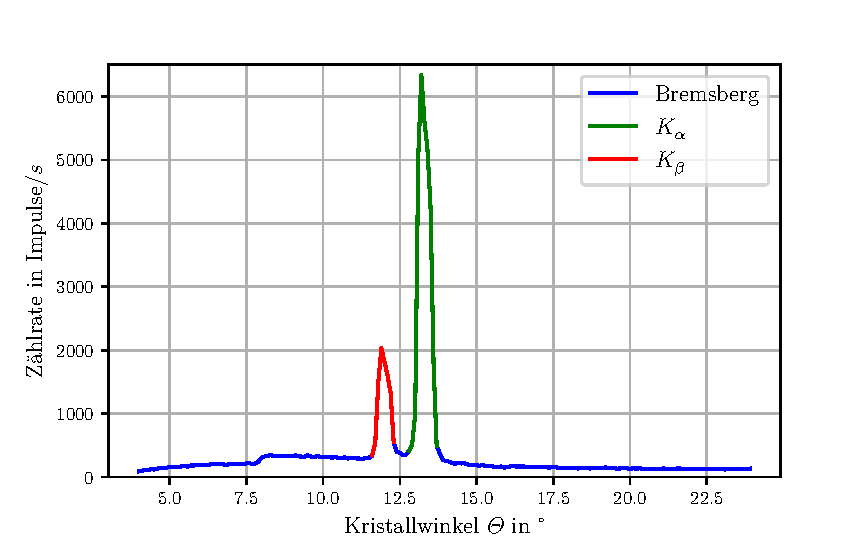
\includegraphics{build/plot_cu.pdf}
  \caption{Emissionsspektrum der Kupfer-Röntgenröhre.}
  \label{fig:cu}
\end{figure}


Das charakteristische Spektrum der Kupfer-Röntgenröhre ist in \autoref{fig:cu} zu sehen.\\
Mit zunehmendem Winkel erkennt man den Grenzwinkel bei  $K_{\alpha}$ und $K_{\beta}$. \\ 
Aus dem Grenzwinkel 
\begin{equation*}
  \theta_{min} = 7,9°
\end{equation*}
lassen sich die maximale Energie und die minimale Wellenlänge 
\begin{equation*}
  E_{max} = 9,137 \mathrm{keV}
\end{equation*}
\begin{equation*}
  \lambda_{min} = 137.5 \si{\pico\m}
\end{equation*} 
berechnen.


\subsubsection*{Auflösungsvermögen der Apparatur}

Mit Hilfe der Halbwertsbreite lässt sich auch das Auflösungsvermögen der Apparatur bestimmen. \\
Die Halbwertsbreite berechnet sich aus den Winkeln $\theta_\beta = 11,9°$ und $\theta_\alpha = 13,2°$.\\
So ergeben sich die Energien zu $E_\alpha = 9,145$ keV und $E_\beta = 8,255$ keV. Aus einem Gaußschen Fit mit Matlab mit der Funktion
\begin{equation*}
  f(x)=a\cdot exp(-((x-b)/c)^2)
\end{equation*} 
ergeben sich mit
\begin{equation*}
  FWHM=2\sqrt{\ln(2)}\cdot c
\end{equation*} 
die Halbwertesbreiten für die jeweiligen K-Linien
\begin{equation*}
  FWHM_{\alpha}=0.4587\ \si{\keV}
\end{equation*}
\begin{equation*}
  FWHM_{\beta}=0.5107\ \si{\keV}
\end{equation*} 
mit denen sich folgende Auflösungsvermögen durch
\begin{equation*}
  A=\frac{E_{\alpha/\beta}}{FWHM_{\alpha/\beta}}
\end{equation*}
berechnet werden können.
Es ergeben sich die Ausflösungsvermögen $\A_{\alpha}=17.9836$ und $\A_{\beta}=17.6305$.\\


\subsubsection*{Abschirmkonstanten}

Aus den berechneten Energien $E_{K \alpha}$ und $E_{K \beta}$ und dem Literaturwert $E_{K,\;abs} = 8980.476 \; \mathrm{eV}$ können die 
Abschirmkonstanten $\sigma_1$, $\sigma_2$ und $\sigma_3$ von Kupfer wie folgt bestimmt werden. Die Ordnungszahl lautet $Z = 29$, $n=1$, $m=2$ und $l=3$. \\
Aus 
\begin{equation*}
  \sigma_1=Z-\sqrt{\frac{E_{Kabs}}{R_\infty}}
  \label{eq:sigma}
  \end{equation*}
  
  \begin{equation*}
  \sigma_2=Z-\sqrt{ \frac{m^2}{n^2}(Z-\sigma_1)^2 - \frac{m^2}{R_\infty} E_{K\alpha}}
  \end{equation*}
  
  \begin{equation*}
      \sigma_3=Z-\sqrt{ \frac{l^2}{n^2}(Z-\sigma_1)^2 - \frac{l^2}{R_\infty} E_{K\beta}}
  \end{equation*}
ergeben sie sich zu $\sigma_1 = 3,30$, $\sigma_2 = 13,57$. 
$\sigma_3$ kann nicht korrekt bestimmt werden, da sich ein komplexer Wert ergibt.




\subsection{Absorptionsspektren}
\label{subsec:absorptionsspektrum}


\subsubsection*{Absorptionsspektrum von Zink}
In \autoref{fig:zink} ist das gemessene Absorptionsspektrum von Zink abgebildet.\\
Darin ist die K-Kante bei $\theta = 11,9°$ zu sehen. \\
Nach \autoref{eq:6} ist die ergibt sich die Absorptionsenergie $E_{Zn, \; K} = 9,138 \mathrm{ keV}$.\\
Daraus lässt sich die Abschirmkonstante $\sigma_{Zn, \; K} = 4,08$ errechnen.
\begin{figure}
  \centering
  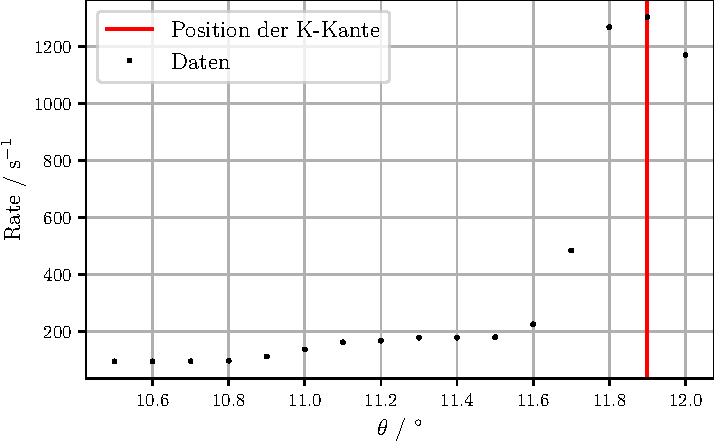
\includegraphics{zink.pdf}
  \caption{Absorptionsspektrum der Röntgenstrahlung von Zink.}
  \label{fig:zink}
\end{figure}


\subsubsection*{Absorptionsspektrum von Gallium}
Im Absorptionsspektrum von Gallium ist die K-Kante bei $\theta = 10,5°$ zu sehen. \\
Nach \autoref{eq:6} ist die ergibt sich die Absorptionsenergie $E_{Ga, \; K} = 10,34 \mathrm{ keV}$.\\
Daraus lässt sich die Abschirmkonstante $\sigma_{Ga, \; K} = 3,43$ errechnen.

\subsubsection*{Absorptionsspektrum von Brom}
Im Absorptionsspektrum von Brom ist die K-Kante bei $\theta = 8,3°$ zu sehen. \\
Nach \autoref{eq:6} ist die ergibt sich die Absorptionsenergie $E_{Br, \; K} = 13,54 \mathrm{ keV}$.\\
Daraus lässt sich die Abschirmkonstante $\sigma_{Br, \; K} = 3,45$ errechnen.

\subsubsection*{Absorptionsspektrum von Strontium}
Im Absorptionsspektrum von Strontium ist die K-Kante bei $\theta = 6,8°$ zu sehen. \\
Nach \autoref{eq:6} ist die ergibt sich die Absorptionsenergie $E_{Sr,\; K} = 15,9  \mathrm{ keV}$.\\
Daraus lässt sich die Abschirmkonstante $\sigma_{Sr, \; K} = 3,81$ errechnen.

\subsubsection*{Absorptionsspektrum von Zirkonium}
Im Absorptionsspektrum von Zirkonium ist die K-Kante bei $\theta = 6,4°$ zu sehen. \\
Nach \autoref{eq:6} ist die ergibt sich die Absorptionsenergie $E_{Zr, \; K} = 16,9  \mathrm{ keV}$.\\
Daraus lässt sich die Abschirmkonstante $\sigma_{Zr, \; K} = 4,75$ errechnen.





\subsubsection*{Moseleysches Gesetz}

Die lineare Ausgleichsrechnung ergibt für die Ausgleichsgerade $y = ax + b$ die Parameter $a = 3,443 \pm 0,2283$ keV und $b = -5,864 \pm 7,9946$ keV.\\
So ergibt sich für die experimentiell bestimmte Rydbergkonstante $R_{exp} = 9,56 \cdot 10^6 \mathrm{\frac{1}{m}}$. 

\begin{figure}
  \centering
  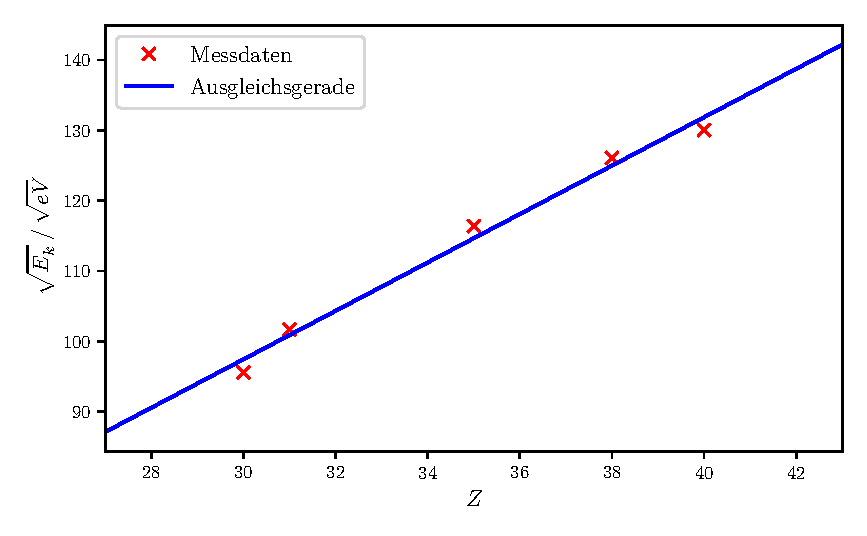
\includegraphics{plot_moseley.pdf}
  \caption{Die Quadratwurzel der Absorptionsenergie in Abhängigkeit von der Ordnungszahl Z mit Ausgleichsgeraden.}
  \label{fig:moseley}
\end{figure}






%\begin{figure}
%  \centering
%  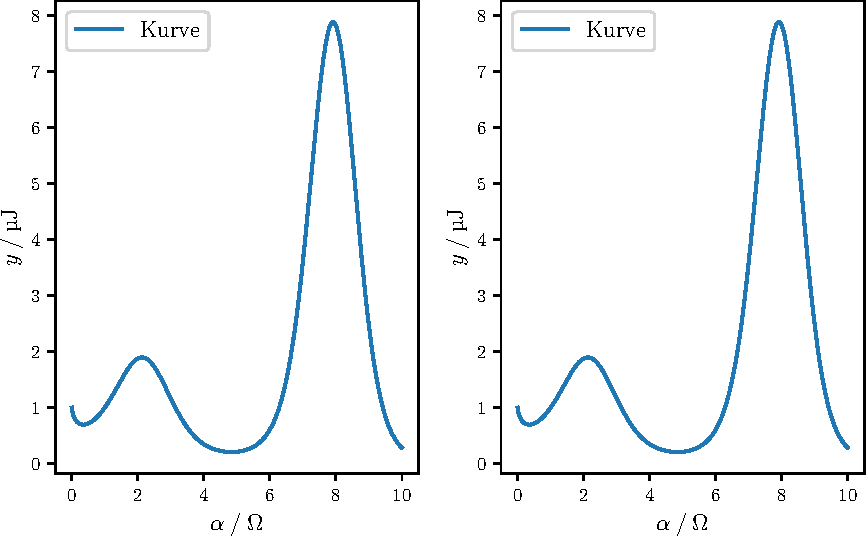
\includegraphics{plot.pdf}
%  \caption{Plot.}
%  \label{fig:plot}
%\end{figure}

%\begin{figure}
%  \centering
%  \includegraphics{build/emissionsspektrum.pdf}
%  \caption{ noch einfügen }
%  \label{fig:plot2}
%\end{figure}



%\begin{figure}
%  \centering
%  \includegraphics{build/moseley.pdf}
%  \caption{Plot.}
%  \label{fig:plot3}
%\end{figure}
%

\section{Diskussion}
Bei den K-Linien weichen die Energien um
\begin{equation*}
  E_{\alpha_{\%}}=2\ \%
\end{equation*}
\begin{equation*}
  E_{\beta_{\%}}=1\ \%
\end{equation*}
und die Winkel um
\begin{equation*}
  \theta_{\alpha_{\%}}=2\ \%
\end{equation*}
\begin{equation*}
  \theta_{\beta_{\%}}=2\ \%
\end{equation*}
ab. Das ist wieder in einem geringen Rahmen und akzeptabel.

\subsection{Überprüfung der Bragg-Bedingung}
Wird der Theoriewert mit dem experimentellen Wert verglichen, ergibt sich zu
\begin{equation*}
  |\frac{\theta_{theo}-\theta_{exp}}{\theta_{exp}}|=0.08\%,
\end{equation*}
woraus sich erkennen lässt, dass die Abweichung sehr gering ist und die Bragg-Bedingung erfüllt.

\subsection{Emissionsspektrum}

\subsection{Absorptionsspektren}
Für die Energien, Winkel und Abschirmkonstanten ergeben sich folgende Abweichungen:
\begin{table}[H]
  \centering
  \begin{tabular}{l|l|l|l}
  & $E_{\%}$ & $\theta_{\%}$ & $\sigma_{\%}$\\ \hline
  Zn & $6\ \%$ & $5\ \%$ & $13\ \%$\\ \hline
  Ga & $7\ \%$ & $7\ \%$ & $7\ \%$\\ \hline
  Br & $1\ \%$ & $4\ \%$ & $12\ \%$\\ \hline
  Sr & $1\ \%$ & $1\ \%$ & $5\ \%$\\ \hline
  Zr & $7\ \%$ & $6\ \%$ & $14\ \%$\\ \hline
  \end{tabular}
  \caption{Die Abweichungen in Prozent.}
\end{table}
Die Abweichungen der Energien und Winkel sind sehr gering, die Abschirmungskonstanten jedoch überschreiten die $10\ \%$-Marke, was vermutlich durch die geringen Abweichungen in den Energien und Winkeln zustande kommt. 

\subsection{Mosleysches Gesetz}
Die theoretische Rydbergkonstante ist $R_{\infty}=1.097\cdot 10^{7}\ \frac{1}{m}$. Im Vergleich mit der experimentellen ergibt sich eine Abweichung von 
\begin{equation*}
  R_{\%}=13\ \%
\end{equation*}
die dadurch erklärbar ist, dass die Konstante mit einer linearen Ausgleichsrechnung berechnet wurde. 

\section{Literaturverzeichnis}
[1] Technische Universität Dortmund, \textit{V602: Röntgenemission und -absorption}






\end{document}